\chapter{Programmazione Non Lineare}

Un generico problema di programmazione non lineare (PNL) sarà descritto nel seguente modo:
\begin{align*}
    &\min f(x)\\
    &x \in X\\
    &x \leq R^n\\
    &f: R^n \rightarrow R
\end{align*}

Prima di continuare con la spiegazione, è bene fare un piccolo ripasso riguardo ai minimi globali e locali di una funzione.

Definiamo un minimo globale:
\[\bar{x} \in X : f(\bar{x}) \leq f(x) \quad \forall x \in X\] 
Un minimo globale stretto si definisce allo stesso modo ma con vincolo di minore stretto e con il vincolo per cui $x \neq \bar{x}$.

Si definisce minimo locale:
\[\bar{x} \in X : \exists I(\bar{x},r),r > 0: f(\bar{x}) \leq f(x) \forall x \in X \cap I(\bar{x},r)\] 
Allo stesso modo di come abbiamo definito il minimo globale stretto, si definisce il minimo locale stretto.

Le possibili cose che possono accadere quando ragioniamo con problemi di ottimizzazione non lineare sono le seguenti:
\begin{itemize}
    \item La funzione obiettivo non è limitata e, in questo caso, la funzione non ha minimo e, quindi, il problema non ha soluzioni.
    \item La funzione obiettivo è limitata ma non ha minimo e, anche in questo caso, non vi è soluzione. Questa cosa può accadere, ad esempio, quando abbiamo un comportamento asintotico verso lo 0.
    \item La funzione obiettivo è limitata e ha minimo.
    \item La funzione obiettivo è definita in un insieme $X$ vuoto. 
\end{itemize}

Possiamo fare una classificazione di questo tipo di problemi in due tipi:
\begin{figure}[H]
    \centering
    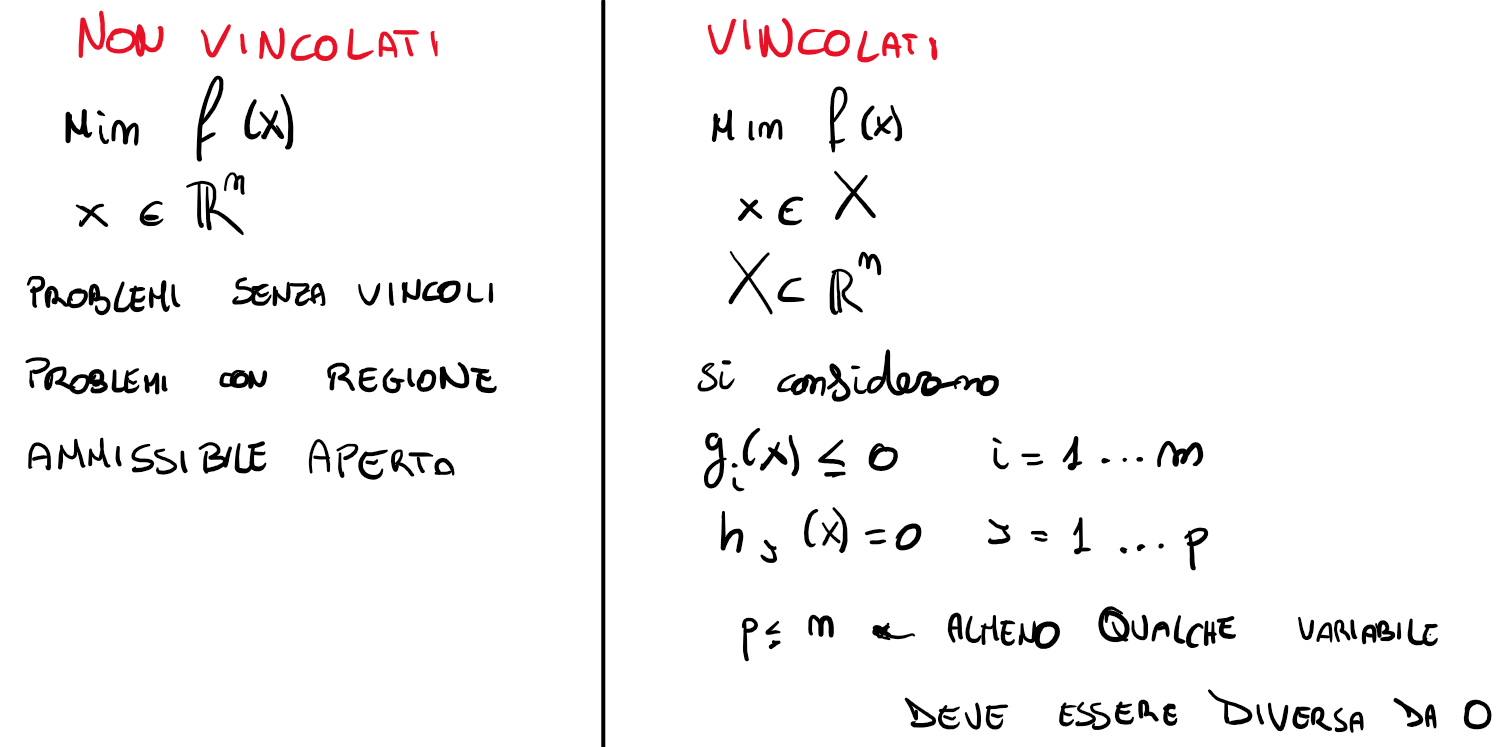
\includegraphics[width=0.7\linewidth]{Images/programmazione_non_lineare/classificazione_vincoli.png}
\end{figure}
Definiamo un vincolo come \textbf{violato} in un punto se $\bar{x} \in R^n: g(\bar{x}) > 0$ dove g è, quindi, un vincolo di minore uguale.
Definiamo un vincolo come \textbf{attivo} in un punto se $\bar{x}:g(\bar{x}) = 0$.

Possiamo effettuare un'altra classificazione che riguarda il fatto che il problema sia o meno convesso:
\begin{figure}[H]
    \centering
    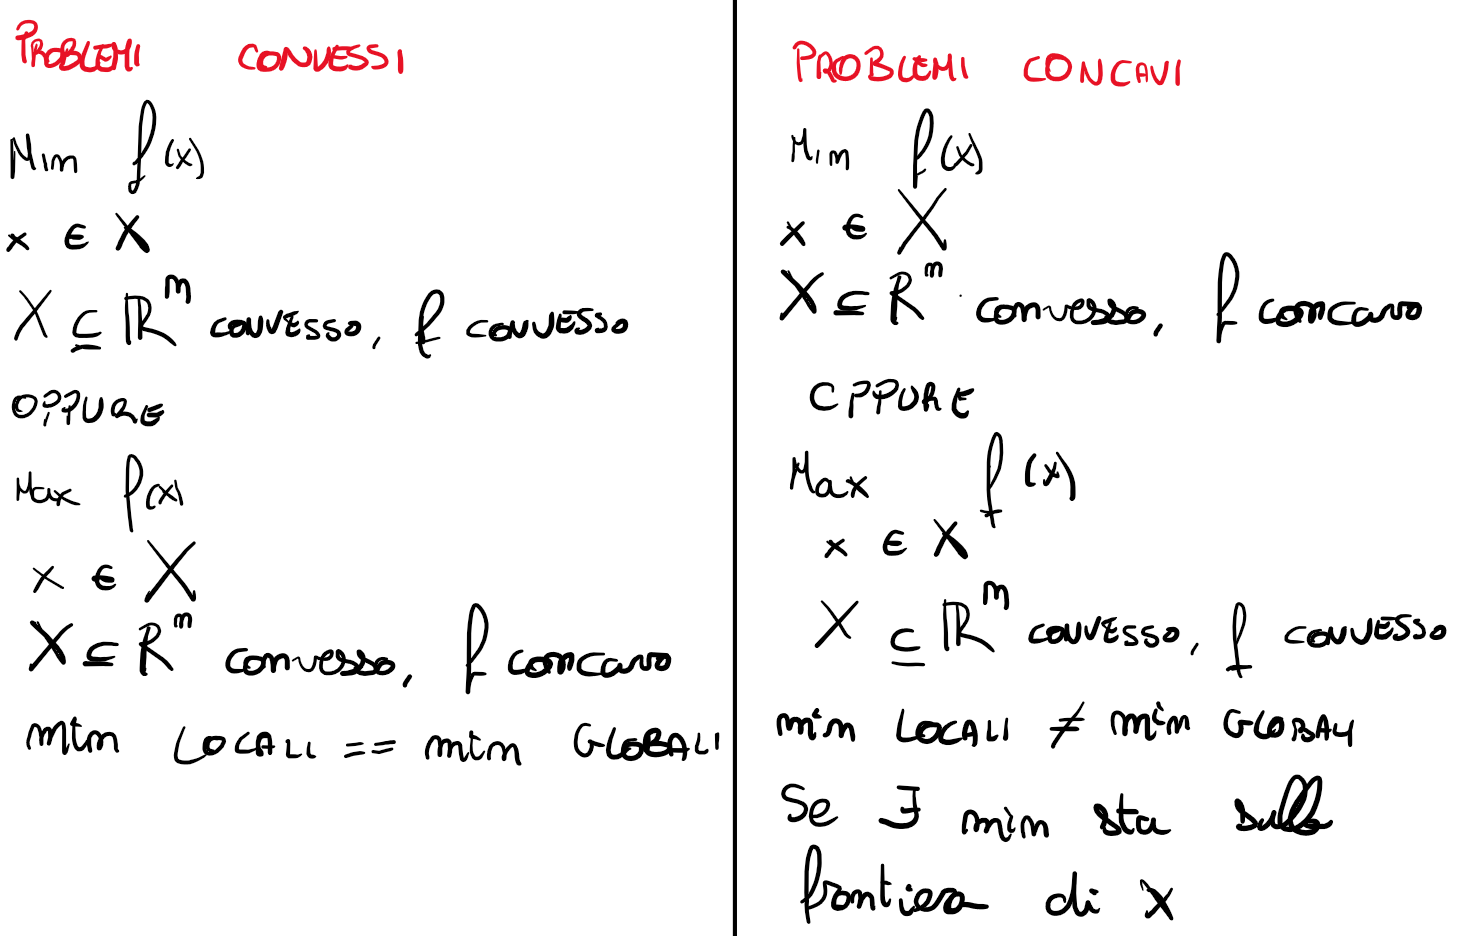
\includegraphics[width=0.7\linewidth]{Images/programmazione_non_lineare/classificazione_convessi_concavi.png}
\end{figure}

\section{Ottimizzazione Non Vincolata}
Quando andiamo a lavorare con problemi di programmazione non lineare non vincolati, abbiamo a che fare con problemi del tipo:
\[\min(f(x) \quad x \in R^n)\]
Per risolvere questo genere di problemi andiamo a cercare dei possibili punti di ottimo mediante delle \textbf{condizioni necessarie}. Questo tipo di condizioni vengono sempre rispettate se $\bar{x}$ è minimo locale ma non è detto che se rispettate, allora $\bar{x}$ sia un ottimo. Una volta trovati i candidati a ottimo, verrà verificata su questi la \textbf{condizione sufficiente}, per cui se vale questa proprietà, allora il punto è sicuramente un ottimo. 

Queste condizioni necessarie si basano sul concetto di direzione di discesa.  Un vettore $d \in R^n$ è una \textbf{direzione di discesa} per f in un punto $\bar{x} \in R^n$ se $\exists \bar{\alpha} > 0: f(\bar{x}+\alpha d) \leq f(\bar{x}) \quad \forall \alpha \in (0, \bar{\alpha})$. Ciò vuol dire che spostando da $\bar{x}$ lungo $d$ di un passo $\alpha$ piccolo, abbassiamo il valore della funzione obiettivo.
\subsection{Condizioni del Primo Ordine}
CN:  Un punto $\bar{x} \in R^n$ è di minimo locale per f se $\nabla f(\bar{x})^T d \geq 0 \quad \forall d \in R^n$. Se $\bar{x}$ è un minimo locale, non possono esistere direzioni di decrescita da quel punto.\\
\textbf{Condizione necessaria del primo ordine}\\
Se $\bar{x} \in R^n$ è un minimo locale per f, allora $\nabla f(\bar{x}) = 0$.

CNS: Sia f convessa.\footnote{Se la matrice Hessiana è semidefinita positiva, allora è f è convessa.} $\bar{x}$ è un minimo globale se e solo se $\nabla f(\bar{x}) = 0$.

\subsection{Condizioni del Secondo Ordine}
CN: Se $\bar{x} \in R^n$ è un minimo locale, vale che:
\begin{itemize}
    \item $\nabla f(\bar{x}) = 0$.
    \item La matrice \textbf{Hessiana} è semidefinita positiva. Una matrice $A$ di ordine $n \times n$ si definisce semidefinita positiva se $d^T Ad > 0, \forall d \in R^n$.
\end{itemize}
Altri modi per capire se una matrice è semidefinita positiva sono:
\begin{figure}[H]
    \centering
    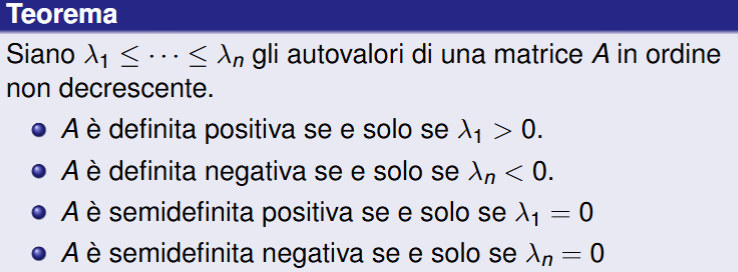
\includegraphics[width=0.6\linewidth]{Images/programmazione_non_lineare/teorema_positivita_hess_1.png}
\end{figure}
\begin{figure}[H]
    \centering
    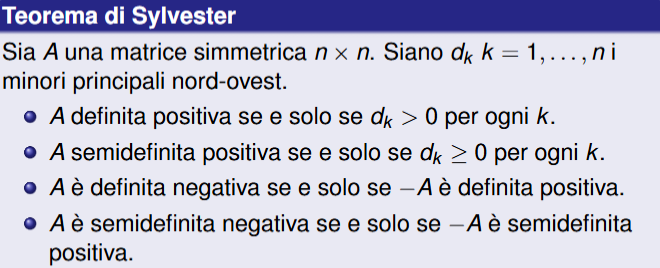
\includegraphics[width=0.6\linewidth]{Images/programmazione_non_lineare/teorema_sylvester.png}
\end{figure}
Dove i \textbf{minori principali nord ovest} sono i determinanti $k \times k$ a partire da in alto a sinistra.
\begin{figure}[H]
    \centering
    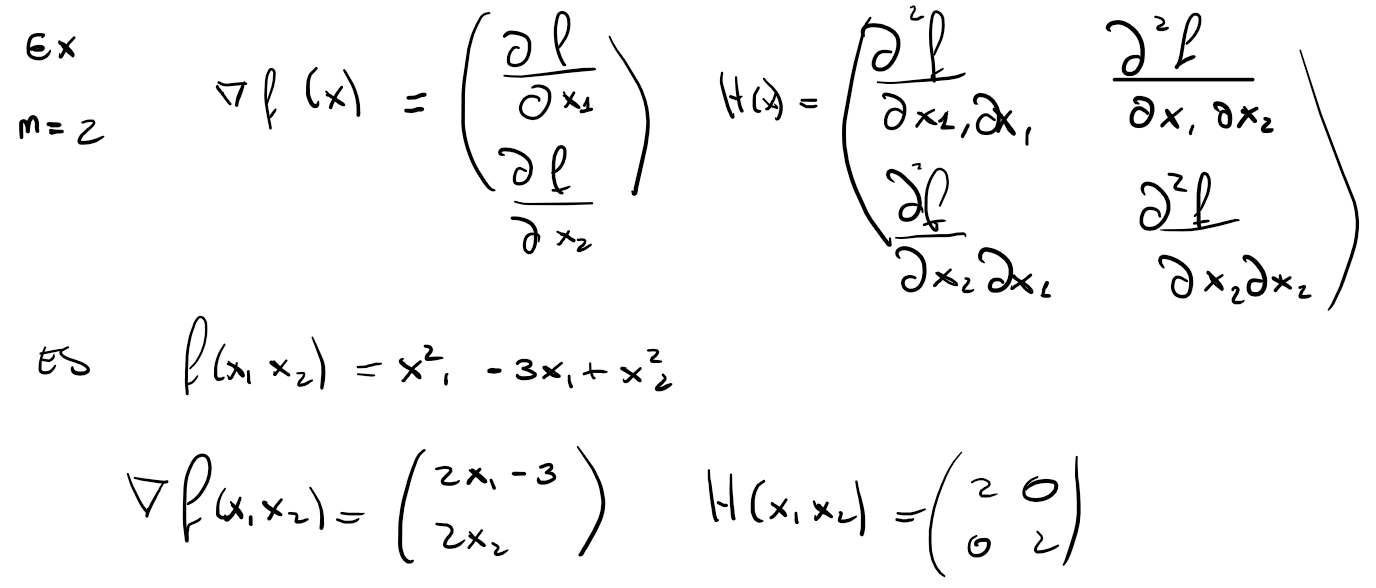
\includegraphics[width=0.6\linewidth]{Images/programmazione_non_lineare/esempio_hessiana.png}
\end{figure}

CS: Se $\nabla f(\bar{x}) = 0$ e se la matrice hessiana è definita positiva, allora $\bar{x}$ è punto di minimo locale.
Ricordiamo che f è convessa se e solo se la matrice hessiana è semidefinita positiva, cioè se $d^T H(x) d \geq 0$ e gli autovalori sono $\geq 0$.


La procedura che seguiamo è:
\begin{enumerate}
    \item Applichiamo CN di ottimalità per trovare i potenziali punti di minimo.
    \item Applichiamo CS di ottimalità per trovare l'ottimo tra i punti trovati con la CN.
\end{enumerate}

Naturalmente, se la funzione è convessa, ci basta la condizione necessaria poiché le condizioni necessarie trovano il punto di minimo locale ma, per funzioni convesse, questo coincide con il minimo globale.

Vediamo un esempio:
\begin{figure}[H]
    \centering
    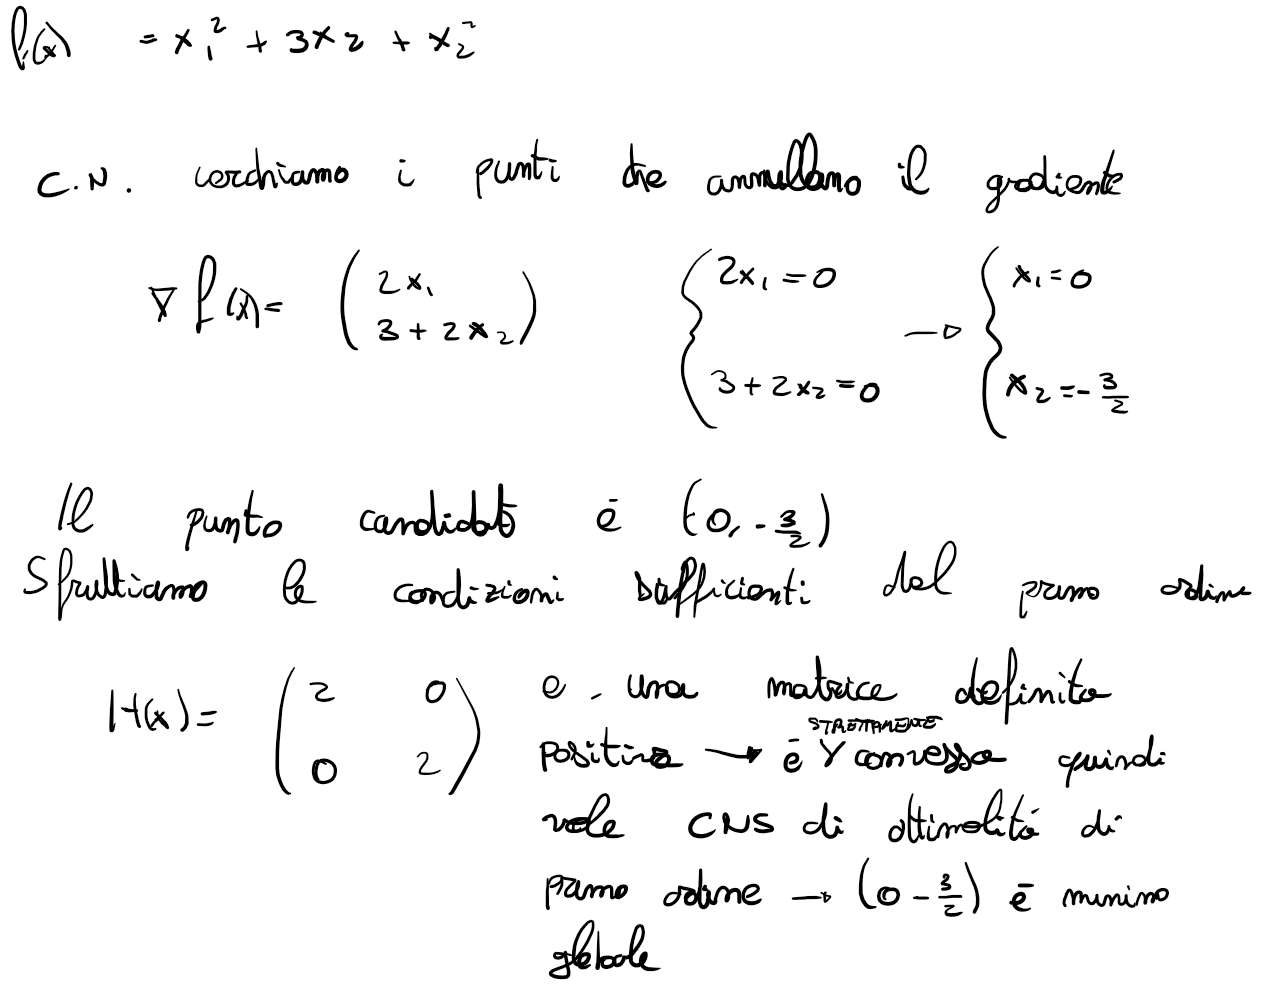
\includegraphics[width=1\linewidth]{Images/programmazione_non_lineare/esempio_senza_vincoli.png}
\end{figure}

\section{Ottimizzazione Vincolata}
Un problema di ottimizzazione vincolata, è un problema del tipo:
\[\min f(x) \quad h_j(x) = 0 \quad g_i \leq 0\]
\subsection{Problemi con Vincoli di Uguaglianza}
Ci concentriamo adesso su problemi con solo vincoli di uguaglianza a 0. 
Sia $\bar{x}$ un punto ammissibile\footnote{Cioè che rispetta i vincoli}, si dice \textbf{regolare per i vincoli} se $\nabla h_j(\bar{x}) : \forall j=1,\dots,p$ sono vettori linearmente indipendenti.

CN: Sia $\bar{x}$ un punto ammissibile e regolare per i vincoli. Se $\bar{x}$ è un punto di minimo locale, allora $\exists \lambda_1, \dots, \lambda_p \in R$:
\[\nabla f(\bar{x})+\sum_{j=1}^p \lambda_j \nabla h_j(\bar{x})=0\]
Dove $\lambda \in R^p$ sono detti \textbf{moltiplicatori di Lagrange}.\footnote{Questa cosa viene fatta creando un sistema con le derivate parziali del Lagrangiano e i vincoli del sistema (messi per far sì che troviamo solo punti ammissibili)} Vediamone un esempio:
\begin{figure}[H]
    \centering
    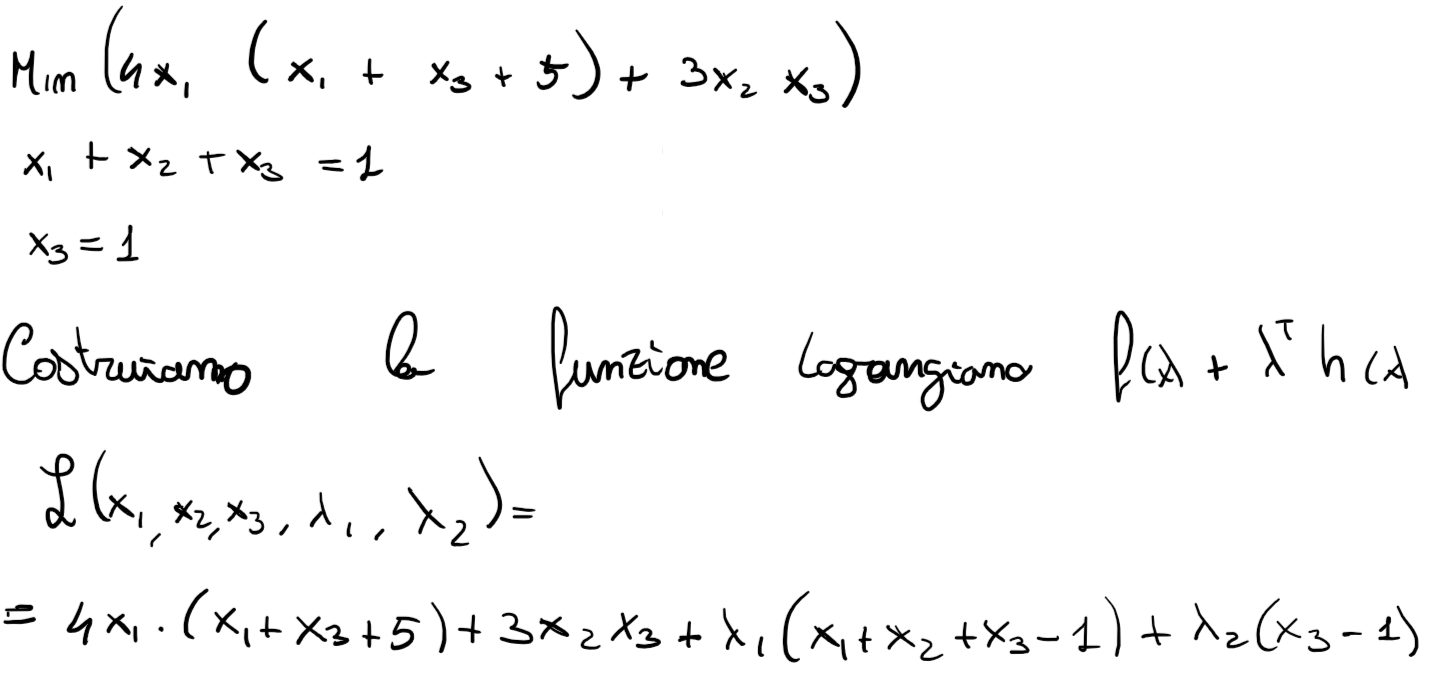
\includegraphics[width=0.7\linewidth]{Images/programmazione_non_lineare/esempio_ottimizzazione_vincolata/1.1.png}
\end{figure}
\begin{figure}[H]
    \centering
    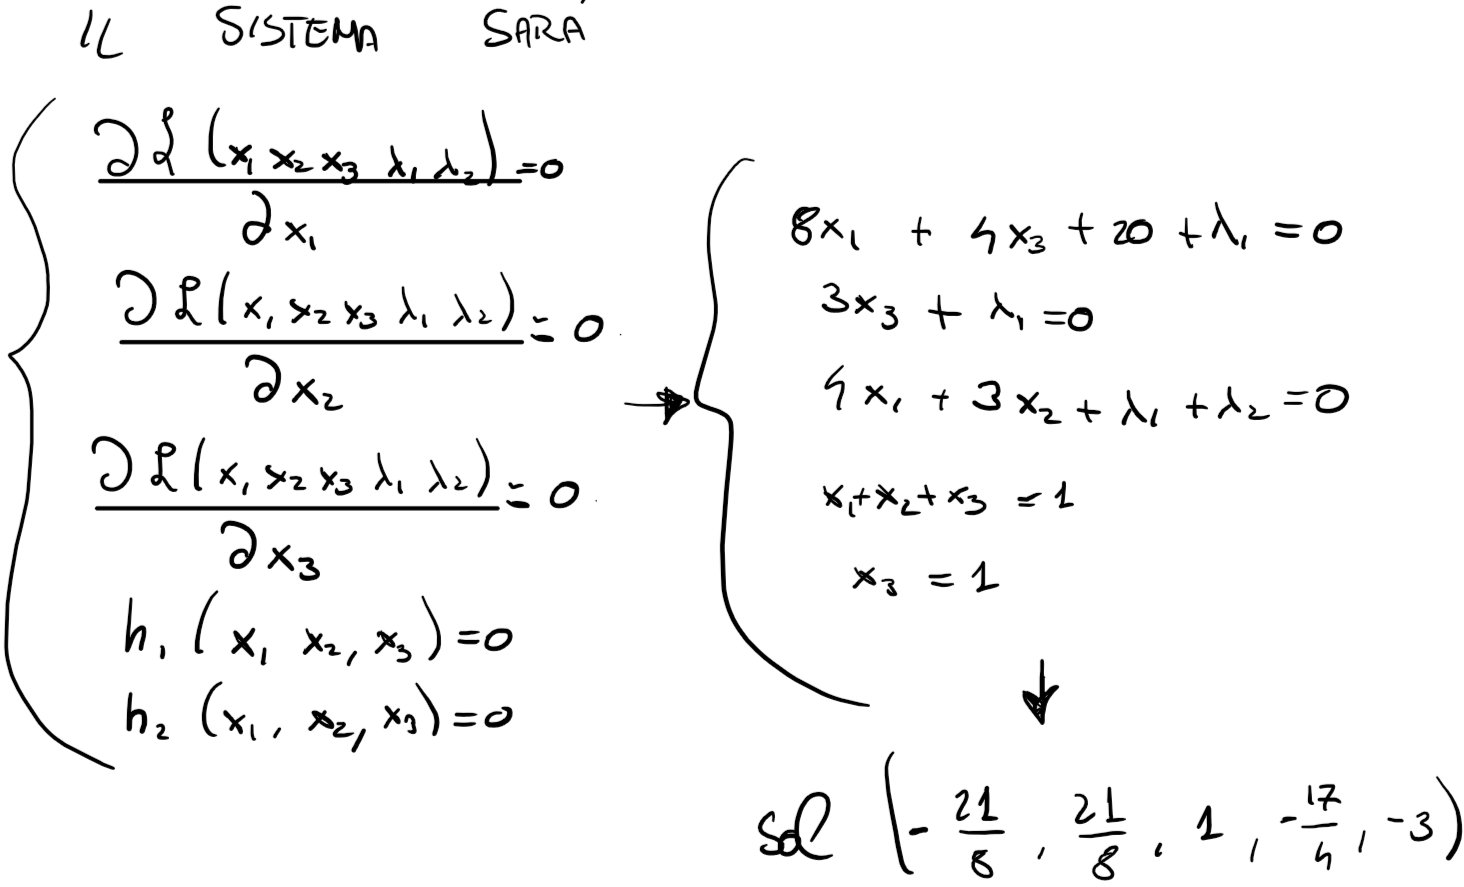
\includegraphics[width=0.7\linewidth]{Images/programmazione_non_lineare/esempio_ottimizzazione_vincolata/1.2.png}
\end{figure}

\subsection{Problemi con Vincoli di Uguaglianza e Minore Uguale}
Vediamo, infine, i problemi con tutti i tipi di vincoli, quindi del tipo:
\[\min f(x) \quad h_j(x) = 0 \quad g_i \leq 0\]
Un punto $\bar{x}$ ammissibile si dice \textbf{regolare per i vincoli} se dato $I$ l'insieme dei vincoli attivi nel punto $\bar{x}$, i gradienti di questi vincoli sono linearmente indipendenti. Ad esempio:
\begin{figure}[H]
    \centering
    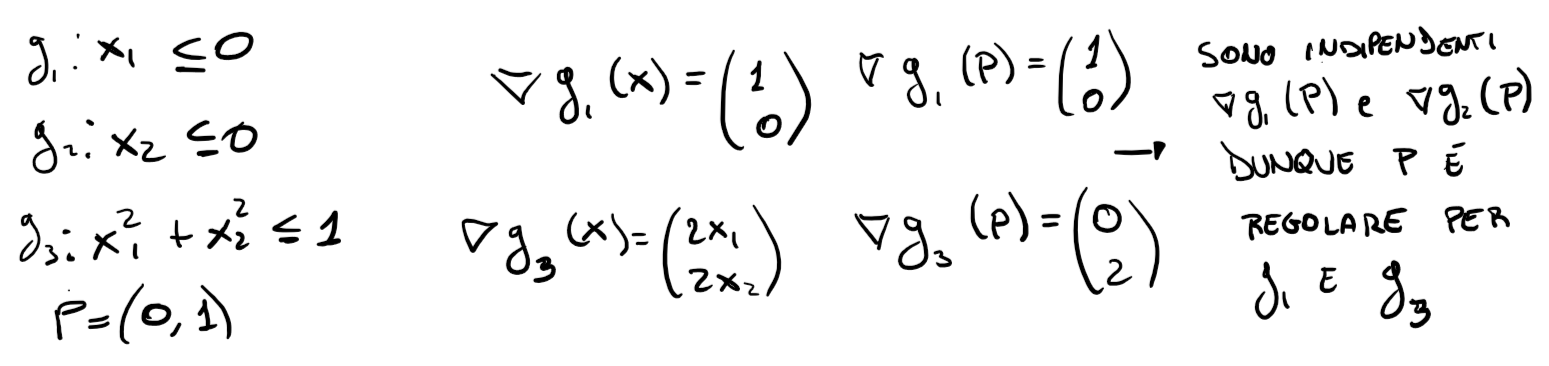
\includegraphics[width=0.7\linewidth]{Images/programmazione_non_lineare/esempio_ottimizzazione_vincolata/2.1.png}
\end{figure}

CN KKT: Sia $\bar{x}$ un punto ammissibile e regolare. Se $\bar{x}$ è un punto di minimo locale, allora $ \exists \lambda_1,
\dots, \lambda_p \in R, \mu_1, \dots, \mu_m \in R_+$ tale che:
\[\nabla f(\bar{x})+\sum_{i=1}^m \mu_i \nabla g_i(\bar{x})+\sum_{j=1}^p \lambda_j \nabla h_j(\bar{x})=0\]
Con:
\begin{align*}
    &\mu_i g_i (\bar{x})= 0 \quad \forall i = 1, \dots, m\\
    &h_j (\bar{x})= 0 \quad \forall j\\
    &g_i (\bar{x})\leq 0 \quad \forall i
\end{align*}

Notiamo come i moltiplicatori $\mu$ dei vincoli di minore uguale devono sempre essere positivi mentre, invece, non abbiamo alcun tipo di vincoli riguardo ai moltiplicatori di uguaglianza.

Inoltre, si sottolinea che se il problema è convesso, allora le condizioni KKT sono necessari e sufficienti di ottimalità.
Vediamo anche qui un esempio:
\begin{figure}[H]
    \centering
    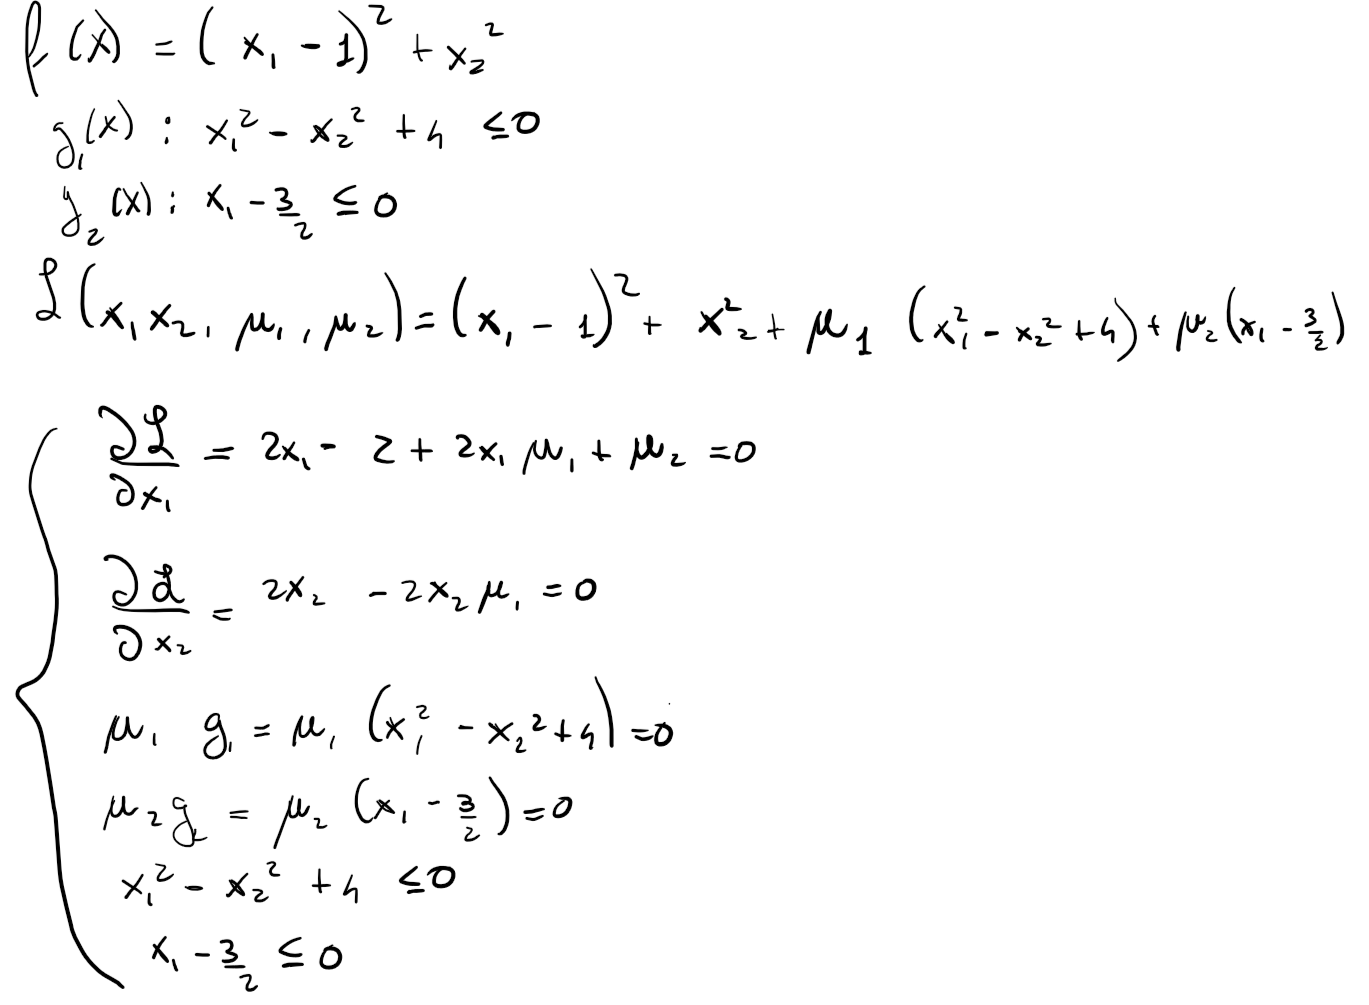
\includegraphics[width=1\linewidth]{Images/programmazione_non_lineare/esempio_ottimizzazione_vincolata/3.1.png}
\end{figure}


\section{Algoritmi di Ottimizzazione Non Vincolata}
I metodi iterativi partono da un punto $x^0 \in R^n$ e generano una successione infinita di punti $\{x^k\}_{k\in N}$ che converge a un punto appartenente all'insieme bersaglio:
\[\Omega : \{x \in R^n: \nabla f(x) = 0\}\]

Tale insieme, nel caso dei problemi non vincolati, coincide con l'insieme dei punti stazionari, cioè quelli per i quali $\nabla f(x) = 0$. I metodi basati sulle direzioni di ricerca individuano, a ogni iterazione, la lunghezza ottimale di
spostamento lungo la direzione di ricerca scelta. Gli algoritmi di questo tipo si dividono in: \textbf{algoritmi senza l’uso di derivate} e \textbf{algoritmi con l’uso di derivate} che saranno quelli che tratteremo adesso. 

In generale quello che facciamo è:
\begin{enumerate}
    \item Scegliamo una soluzione ammissibile $x^0$ e si pone $k=0$.
    \item Se la soluzione $x^k$ verifica una condizione di arresto (cioè $\nabla f(x^k)=0$), ci fermiamo, altrimenti, scegliamo una \textbf{direzione $d^k$}.
    \item Si sceglie un passo $\alpha^k$.
    \item Si pone $x^{k+1}= x^k+\alpha^k d^k$.
    \item Poniamo $k=k+1$ e ripartiamo dal passo 2.
\end{enumerate}

In particolare, ci concentreremo sui \textbf{metodi di discesa}, per cui $f(x^k+\alpha^k d^k) < f(x^k)$.
Iniziamo cercando di capire come scegliere il \textbf{punto $x^0$} anche se, in realtà, non vi è una regola ben definita:
\begin{itemize}
    \item Si può scegliere come $x^0$ il punto stazionario di una funzione obiettivo semplificata.
    \item Si può avviare il metodo a partire da punti diversi e si sceglie il punto stazionario migliore, cioè quello che dà il valore più basso della funzione obiettivo. 
\end{itemize}

Per quanto riguarda la \textbf{direzione $d^k$}, può essere scelta in vari modi e, in realtà, questa scelta determina il metodo che adotteremo.

Infine, il \textbf{passo $\alpha^k$} va' bilanciato in maniera opportuna poiché se troppo lungo rischiamo di saltare il minimo locale, altrimenti facciamo troppe iterazioni.  Può essere ricercato in maniera \textbf{esatta} o \textbf{inesatta}:
\begin{itemize}
    \item La ricerca esatta si usa solo per \textbf{funzioni quadratiche} del tipo $(\frac{1}{2} x^T Qx + b^Tx)$ e consiste nel risolvere un problema di ottimizzazione per trovare il passo ottimale. Si costruisce la funzione $\phi (\alpha) = f(x^k + \alpha d^k)$ e l'$\alpha$ ottimo risolve il problema di minimizzare $\phi(\alpha)$. Quando facciamo la derivata $\phi'(\alpha) = \nabla f(x^k + \alpha d^k)^T d^k = 0$ risulta che la direzione di ricerca $d^k$ è ortogonale al gradiente di f in $x^{k+1}$.
    \item La ricerca inesatta prevede di imporre condizioni su $\alpha^k$ per individuare intervalli  buoni per la scelta del passo che garantiscono una sufficiente riduzione del valore della funzione obiettivo. Anche questo tipo di ricerca, sarà generalmente dettata dal metodo che consideriamo.
\end{itemize}

Per quanto riguarda i \textbf{criteri di arresto} possiamo imporre $\nabla f(x^k) < \epsilon_1$ anche se spesso si aggiungono condizioni del tipo $|| k^{k+1}- x^k||< \epsilon_2$ o $|f(x^k+1) -f(x^k)| < \epsilon_3$. Un ulteriore cosa che si può fare è fissare il numero massimo di iterazioni che possono avvenire.

\subsection{Metodo del Gradiente}
Questo metodo, utilizza come direzione di discesa $d^k=-\nabla f(x^k)$. La generica iterazione sarà $x^{k+1} = x^{k} - \alpha^k \nabla f(x^k)$ con scelta opportuna del passo $\alpha^k$. 

Se si adotta la ricerca esatta di $\alpha^k$, allora $\phi(\alpha) = f(x^k - \alpha^k \nabla f(x^k))$ e facendo poi $\min \phi(\alpha)$, si trova $\phi' (\alpha) = 0 $ che vuol dire che $\nabla f(x^k -\alpha \nabla f(x^k))^T = 0$\footnote{In realtà il - presente nella formula è praticamente dovuto al fatto che la seconda parte incorpora la direzione di discesa} cioè $\nabla f(x^{k+1})^T \nabla f(x^k) = 0$. Ciò vuol dire che le direzioni successive sono ortogonali tra loro. In generale il metodo converge lentamente e ha andamento a zig-zag.
\begin{figure}[H]
    \centering
    
\includegraphics[width=0.8\linewidth]{Images/programmazione_non_lineare/medoto_del_gradiente/1.png}
\end{figure}
\begin{figure}[H]
    \centering
    
\includegraphics[width=0.8\linewidth]{Images/programmazione_non_lineare/medoto_del_gradiente/2.png}
\end{figure}

\subsection{Metodo di Newton}
La funzione f da minimizzare viene approssimata localmente da una funzione quadratica. La funzione f è approssimata dalla
funzione $\phi(x)$ che si ottiene dallo sviluppo in serie di Taylor di $f(x)$ arrestato ai termini di secondo ordine.
Poniamo il passo di Newton $s= \alpha^k d^k$. Dopodiché la funzione sarà:
\[q^k(s) \approx f(x^k + s) \approx f(x^k) + \nabla f(x^k)^T s + \frac{1}{2} s^T \nabla^2 f(x^k) s\]

Ne segue che il passo ottimo di Newton è:
\[s^k=-\nabla f(x^k)[H(x^k)]^{-1}\]\footnote{In realtà l'ordine dovrebbe essere invertito, cioè dovrebbe essere l'inverso moltiplicato meno il gradiente, tuttavia la prof lo ha scritto così ma è necessario considerare il gradiente come un vettore riga.}
Purtroppo, soprattutto a causa del calcolo della matrice Hessiana e della sua inversa, l'uso di questo metodo risulta parecchio oneroso. Dunque, si preferiscono metodi detti \textbf{quasi-newtoniani} che fanno uso di matrici che approssimano l'inversa della matrice Hessiana. In ogni caso, il metodo classico ha convergenza quadratica e converge localmente. Si può far convergere globalmente modificando il metodo assumendo che la direzione sia di discesa e usando l'opposto del gradiente se la matrice Hessiana non è invertibile. Un'applicazione pratica di questo metodo la si può vedere nel problema del best data fitting.
\begin{figure}[H]
    \centering
    
\includegraphics[width=0.8\linewidth]{Images/programmazione_non_lineare/metodo_newton/1.png}
\end{figure} 

\section{Algoritmi per Ottimizzazione Vincolata}
Consideriamo il problema di minimizzazione $\min f(x)$ definito sull'insieme $X \subseteq \mathbb{R}^n$.
La strategia risolutiva dipende dalla natura topologica di $X$:
\begin{itemize}
    \item Se $X$ è un insieme aperto, il problema può essere trattato localmente come non vincolato. Poiché ogni punto di $X$ è un punto interno, i vincoli non sono attivi nelle vicinanze del minimo locale. Di conseguenza, restano valide le condizioni classiche di ottimalità (come l'annullamento del gradiente, $\nabla f(x) = 0$) e si possono applicare gli algoritmi di discesa tipici dell'ottimizzazione libera.
    \item Se $X$ è un insieme chiuso, il minimo potrebbe trovarsi sulla frontiera della regione ammissibile. In questo scenario è necessario utilizzare gli strumenti dell'ottimizzazione vincolata per gestire i vincoli attivi. Si ricorre quindi al metodo dei moltiplicatori di Lagrange (per vincoli di uguaglianza) o alle condizioni di Karush-Kuhn-Tucker (KKT) (per vincoli di disuguaglianza e misti).
\end{itemize}
Il problema più generale sarà:
\[\min f(x) \quad h(x) = 0 \quad g(x)\leq 0\]

Con $f:R^n \rightarrow R$, $g: R^n \rightarrow R^m$ e $h:R^n \rightarrow R^p$ con g e h funzioni continue che garantiscono la chiusura della regione ammissibile.
Per risolvere il problema vincolato senza risolverlo analiticamente, si ricorre a metodi risolutivi che si basano su due approcci:
\begin{enumerate}
    \item Si trasforma il problema vincolato in un problema non vincolato o in una successione di problemi non vincolati.
    \item Si riduce il problema a uno più semplice ma sempre vincolato per poi risolverlo con il metodo del gradiente proiettato.
\end{enumerate}

\subsection{Metodi di Penalità}
Si tratta di un metodo del tipo 1 che trasforma il problema vincolato in uno non vincolato. Sia dato il problema:
\[\min f(x) \quad X:(g(x)\leq 0 \cap h(x)=0)\]
Si risolve il problema non vincolato:
\[\min_{X\in R} f(x)+\alpha \phi(x)\]
Dove $\alpha$ è un parametro di penalità positivo e $\phi(x)$ è la funzione di penalità che punisce la violazione dei vincoli, cioè: 
\begin{align*}
    &\phi(x) > 0 \text{ se $x \notin X$}\\
    &\phi(x) = 0 \text{ se $x \in X$}
\end{align*}
Le funzioni di penalità sono dette esterne perché si parte da punti non ammissibili e ci si avvicina alla frontiera dove si trova l'ottimo.
\begin{figure}[H]
    \centering
    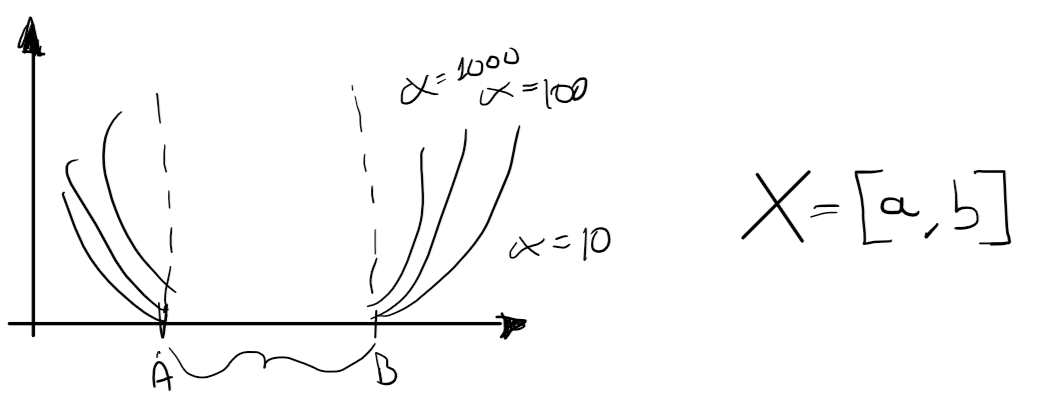
\includegraphics[width=0.5\linewidth]{Images/programmazione_non_lineare/funzione_penalita_alfa.png}
\end{figure} 
Le funzioni di penalità si distinguono in \textbf{sequenziali} ed \textbf{esatte} a seconda della scelta di $\phi(x)$.

Se scegliamo una funzione di \textbf{penalità sequenziale}, allora:
\[\phi(x) = \sum_{i=1}^m [\max\{0,g_i(x)\}]^2+ \sum_{j=1}^p [h_j(x)]^2\]
La funzione $\phi(x)$ è differenziabile. Non esiste uno specifico valore di $\alpha$ per cui i punti stazionari del problema non vincolato coincidono con i punti KKT, tuttavia, si può dimostrare che $\lim_{\alpha \rightarrow \infty}$ soluzione del problema non vincolato dà la soluzione ottima del problema vincolato. Vediamo un esempio di come si costruisce questo tipo di problema e uno di come si risolve a tutti gli effetti:
\begin{figure}[H]
    \centering
    
\includegraphics[width=0.7\linewidth]{Images/programmazione_non_lineare/metodo_della_penalità/1.1.png}
\end{figure} 
\begin{figure}[H]
    \centering
    
\includegraphics[width=0.7\linewidth]{Images/programmazione_non_lineare/metodo_della_penalità/2.1.png}
\end{figure} 
\begin{figure}[H]
    \centering
    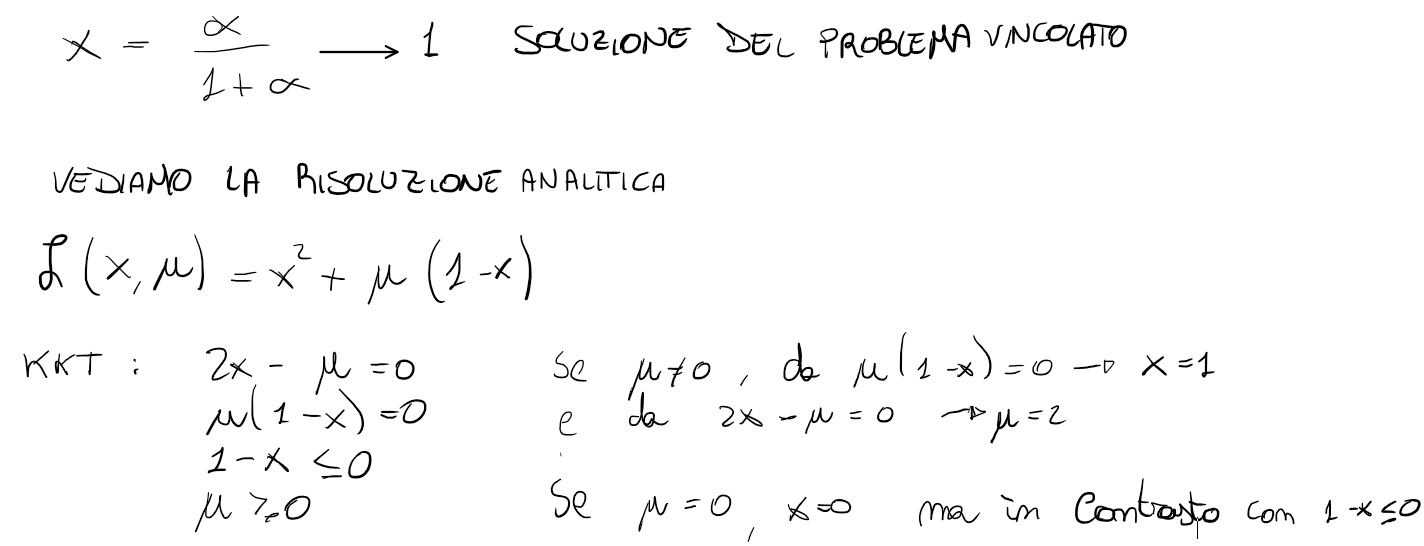
\includegraphics[width=0.7\linewidth]{Images/programmazione_non_lineare/metodo_della_penalità/2.2.png}
\end{figure} 

Per quanto riguarda le funzioni di penalità esatte, si sceglie:
\[\phi(x)= \sum_{i=1}^m \max\{0,g_i(x)\}+\sum_{j=1}^p |h_j(x)|\]
In questo caso, la funzione $\phi(x)$ non è differenziabile. Esiste un valore del parametro $\alpha$ abbastanza grande per cui i punti stazionari del problema non vincolato sono soluzione del problema vincolato. Vediamone un esempio:
\begin{figure}[H]
    \centering
    
\includegraphics[width=0.85\linewidth]{Images/programmazione_non_lineare/metodo_della_penalità/3.1.png}
\end{figure} 

\section{Funzioni Barriera}
L'idea alla base di questo metodo è quella di cercare l'ottimo partendo da punti interni della regione ammissibile, penalizzando quando ci si avvicina alla frontiera. Si lavora, dunque con problemi che hanno interno non vuoto  del tipo:
\[\min f(x) \quad g(x)\leq 0 \quad interno(X)=\{x\in R: g(x)<0\}\neq 0\]
\begin{figure}[H]
    \centering
    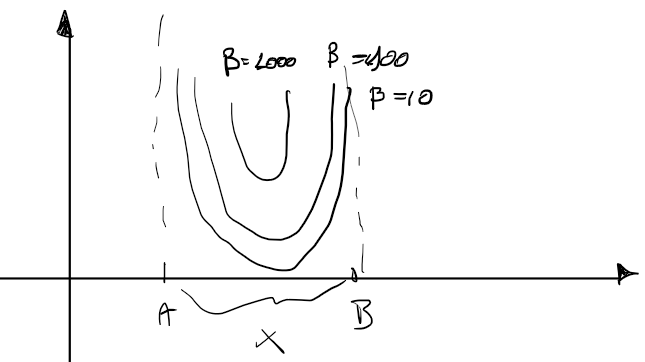
\includegraphics[width=0.5\linewidth]{Images/programmazione_non_lineare/esempio_barriera.png}
\end{figure} 
Si costruisce una funzione barriera $\psi(x)$ e si risolve il problema non vincolato:
\[\min_{x\in R^n}(f(x)+\beta \psi(x)) \quad \beta > 0\]

Per $\lim_{\beta \rightarrow 0}$ la soluzione del problema non vincolato è soluzione del problema vincolato. Tipicamente possiamo scegliere $\psi (x)$ come:
\begin{itemize}
    \item \textbf{Barriera inversa:} 
    $-\sum^m \frac{i}{g_i(x)}$
    \item \textbf{Barriera logaritmica:} $-\sum^n \log(-g_i(x))$
\end{itemize}
Vediamo un esempio:
Un drone ottimizza tempo e consumo per visitare due stazioni:
\begin{itemize}
    \item Batteria max: 8 minuti
    \item Volo sicuro almeno 2 minuti per tratta
\end{itemize}
\begin{figure}[H]
    \centering
    
\includegraphics[width=0.9\linewidth]{Images/programmazione_non_lineare/metodo_barriera/1.png}
\end{figure} 
\begin{figure}[H]
    \centering
    
\includegraphics[width=0.6\linewidth]{Images/programmazione_non_lineare/metodo_barriera/2.png}
\end{figure} 
\section{Problemi di classificazione}
Siano $A, B \subseteq R^n$ con $A$ e $B$ disgiunti, cioè: $A \cap B = 0$. $A$ e $B$ siano linearmente separabili, cioè esiste un iperpiano $H:{x\in R^n: w^Tx+b=0}$ che separa elementi di $A$ da elementi di $B$. 
\begin{figure}[H]
    \centering
    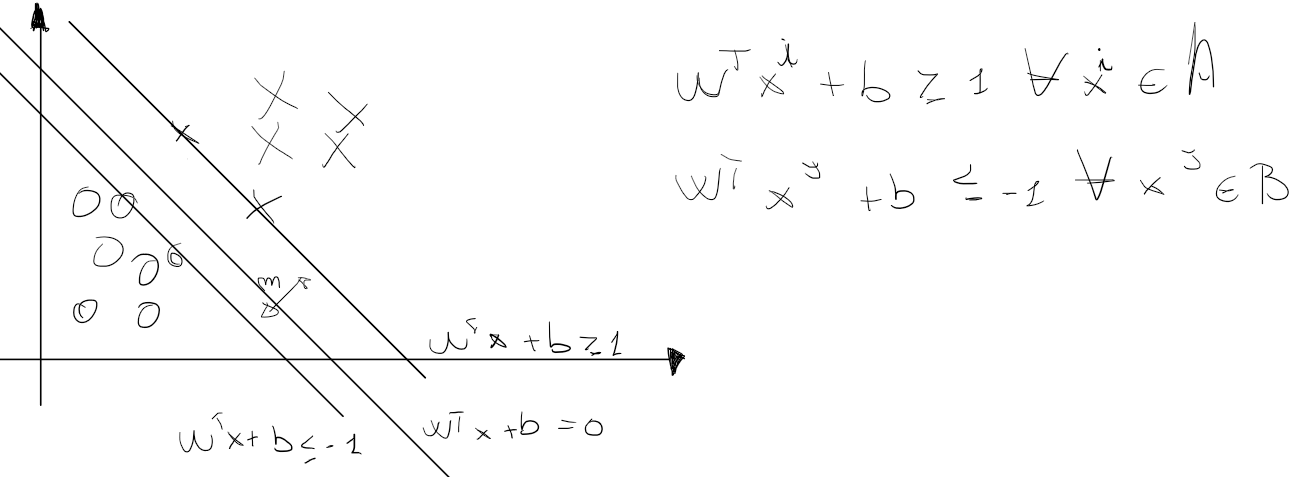
\includegraphics[width=0.6\linewidth]{Images/programmazione_non_lineare/separazione.png}
\end{figure} 

Sia $m$ il margine di separazione:
\[m = \min_{x\in A\cup B} \frac{|w^Tx+b|}{||w||}\]
Se vogliamo, invece, il margine massimo, lo otteniamo come:
\[\max_{w\in R^n, b\in R}\min_{x\in A\cup B} \frac{|w^Tx+b|}{||w||}\]
Il problema equivale a: 
\begin{align*}
    &\min \frac{1}{2} || w||^2\\
    &1-y_i(w^Tx^i+b)\leq 0 \quad \forall i= 1,\dots, p \quad p = |A \cup B|\\
    &y_i = 1 \quad \text{se $x^i \in A$}, y_i= -1 \quad \text{se $x^i \in B$}
\end{align*}
Le condizioni KKT saranno:
\begin{align*}
    &L(w,b,\mu)=\frac{1}{2}||w||^2 + \sum_{i=1}^p \mu_i(1-y_i (w^Tx^i - b))\\
    &\frac{\partial \mathcal{L}}{\partial w_1} = 0, \quad
    \frac{\partial \mathcal{L}}{\partial w_p} = 0, \quad
    \frac{\partial \mathcal{L}}{\partial b} = 0\\
    &\mu_i ( 1 - y_i (w^T x^i + b)) &= 0 \quad \forall i \\
    &1 - y_i (w^T x^i + b) &\leq 0 \\
    &\mu_i &\geq 0
\end{align*}
\begin{figure}[H]
    \centering
    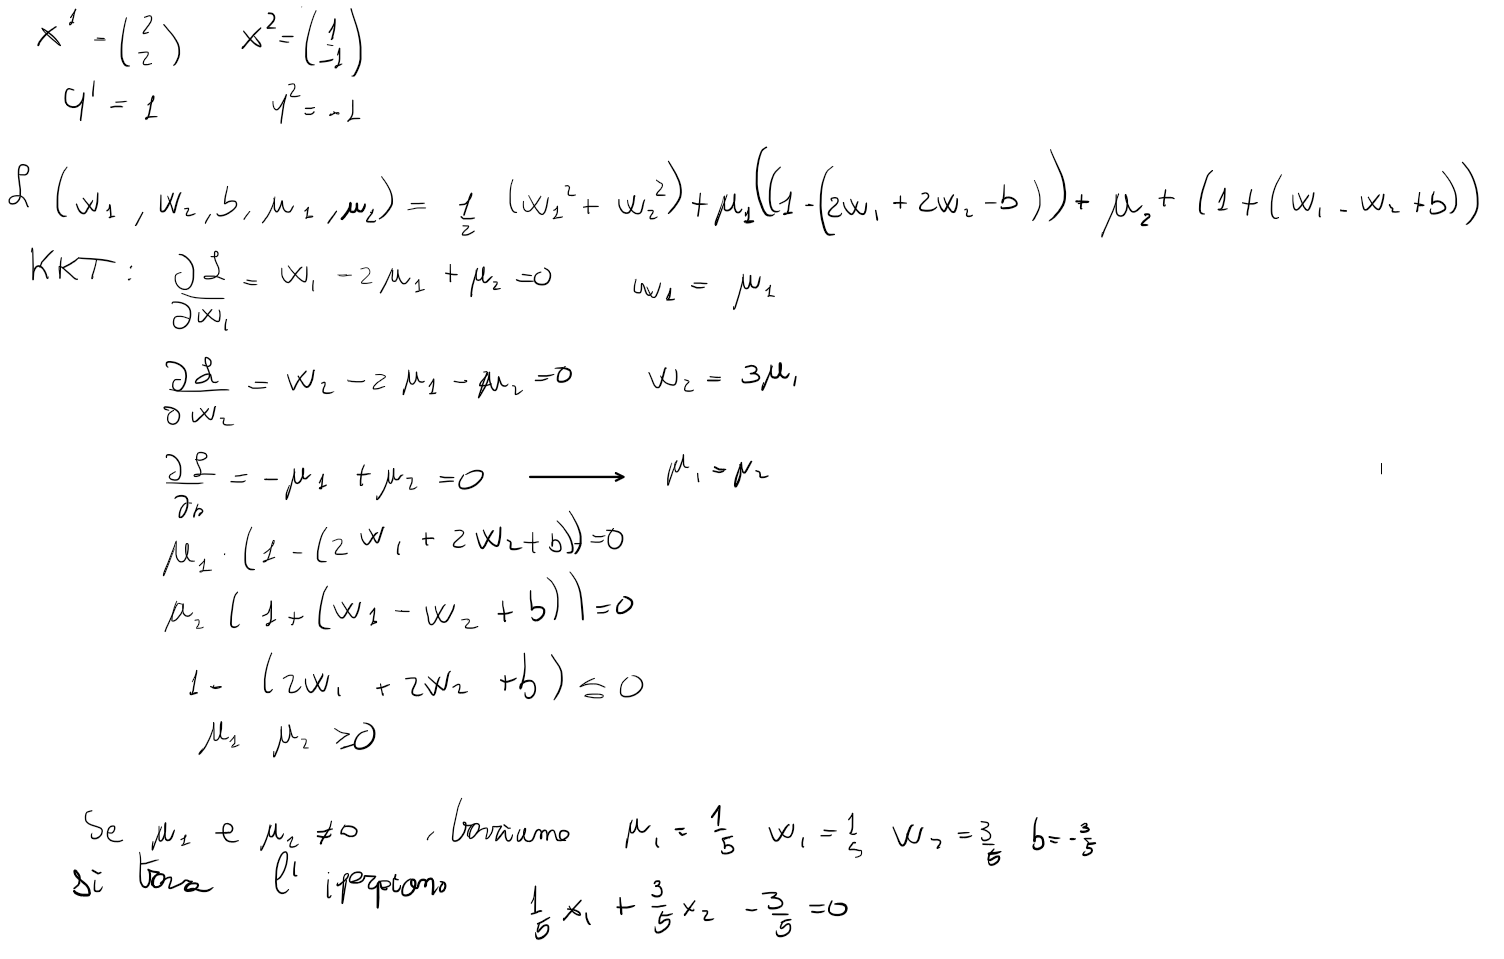
\includegraphics[width=1\linewidth]{Images/programmazione_non_lineare/esempio_separazione.png}
\end{figure} 
